% for landscape posters, use "a4paper, landscape"
\documentclass[a4paper, landscape]{article}
\usepackage{better_poster}


% ---- fill in from here
% poster size - this will scale the poster to the given size.
% for landscape posters add ", landscape" to the postersize command.
\postersize{a0paper, landscape}

% authors
\title{Accelerating the use of Lagrangian data with Clouddrift}
\author{Shane Elipot, Philippe Miron, Milan Curcic, Kevin Santana}

% type of poster: [exp]erimental results, [methods], [theory]
% Disclaimer: the original classification had "study" and "intervention" as separate categories. I group them under experimental results.
\newcommand\postertype{methods} % [exp],[methods],[theory]

\begin{document}

% main point of your study
\makefinding{
Organizing \textbf{lagrangian datasets} into \textbf{ragged arrays} eases data engineering and analysis!
}

% the main text of your poster goes here
\makemain{
    \raggedcolumns
    \begin{multicols}{2}
        \section{Introduction}
        \begin{compactitem}
            \item Lagrangian data sometimes refers to oceanic and atmosphere information acquired by observing platforms drifting within the flow they are embedded in.
        \end{compactitem}

        \section{Datasets}
        \begin{compactitem}
            \item MoSAiC, sea ice trajectories
            \item GDP, ocean drifter trajectories
            \item HURDAT2, cyclone trajectories
            \item Many more...
        \end{compactitem}

        \columnbreak

        \section{Scope / Features}
        \begin{compactitem}
            \item Working with trajectories of varying length
            \item Provide functions and methods for scientific analysis of Lagrangian data
            \item Process publicly available Lagrangian datasets into ragged array zarr archives
            \item Making cloud-optimized ragged array datasets easily accessible
        \end{compactitem}

        % \columnbreak

        \section{Data Structure}
        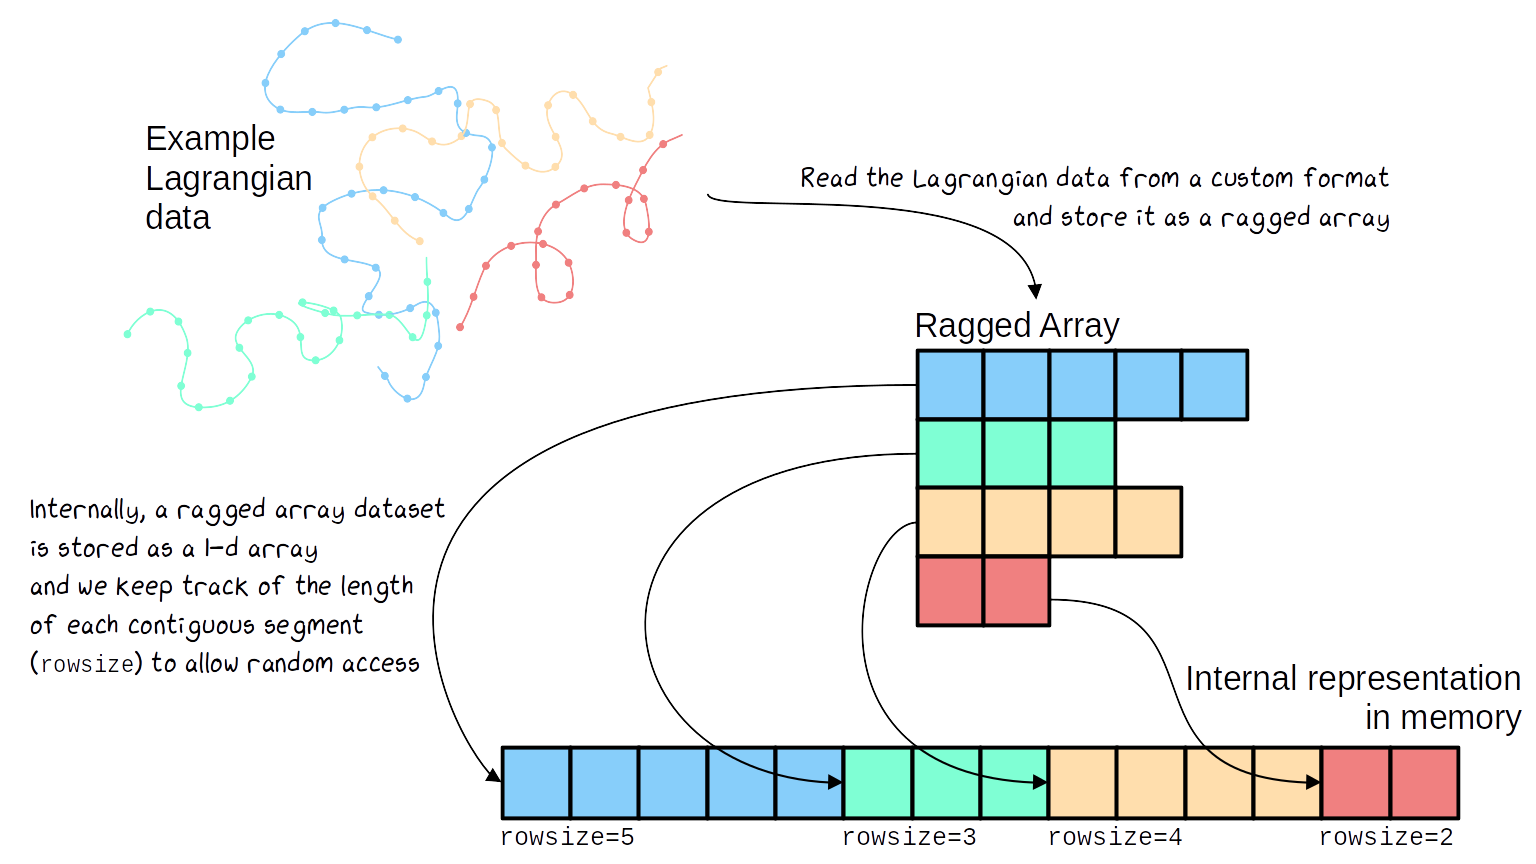
\includegraphics[width=0.35\textwidth, height=0.18\textheight]{ragged-array.png}
    \end{multicols}
}

% footer
% generate qr code from https://www.qr-code-generator.com/ and replace qr_code.png
% default: barcode on the left
\makefooter{images/um-logo.png}{images/qr-code.png}

% replace with this like for barcode on the right
% \makealtfooter{images/qr-code.png}
 
\end{document}
